\documentclass{dhnbpub}

\addbibresource{references.bib}

\sloppy

\usepackage{tikz}
\usetikzlibrary{positioning,arrows.meta}

\begin{document}

\copyrightyear{2027}
\copyrightclause{Copyright for this paper by its authors.
  Use permitted under Creative Commons License Attribution 4.0 International (CC BY 4.0).}

\conference{DHNB2027: Human(ities) in the Loop, March 1--5, 2027, Ume{\aa}, Sweden}

\title{How Much Image Is Enough? Keeping Humans in the Loop of Image Download Infrastructure}

\author[1]{Aram Karimi}
\cormark[1]
\address[1]{Gothenburg Research Infrastructure in Digital Humanities (GRIDH), University of Gothenburg, Sweden}

\author[1]{Jonathan Westin}[%
email=jonathan.westin@lir.gu.se,
]

\author[1]{Tristan Bridge}[%
email=tristan.bridge@gu.se,
]

\author[1]{Julia Beck}[%
email=julia.beck@lir.gu.se,
]

\cortext[1]{Corresponding author.}

\begin{abstract}
  Research infrastructures in the digital humanities increasingly hold
  documentation-grade images whose resolution far exceeds what most
  scholarly tasks require. Deep-zoom viewers make such images explorable
  in the browser, but researchers also need files they can keep,
  annotate, publish and teach with, and the original files are often too
  large to hand out safely or usefully. This paper describes how the
  Gothenburg Research Infrastructure in Digital Humanities (GRIDH)
  approached this problem by building a small on-demand download service
  that lets a person choose between three resolution levels of an image,
  generates the requested derivative only once, and stores it in
  project-scoped public storage. We present the design as a set of
  negotiations between what is safe and easy for the people who use the
  material and what is safe and efficient for the people who maintain
  the infrastructure. We argue that the question ``how much image is
  enough?'' is an interpretive, humanistic judgement that should stay
  with a human, and that infrastructures can be designed so that this
  judgement is visible, cheap to exercise and bounded in its
  consequences. We close with an account of the limitations of the
  current prototype.
\end{abstract}

\begin{keywords}
  research infrastructure \sep
  image derivatives \sep
  IIIF \sep
  human in the loop \sep
  sustainability \sep
  cultural heritage data
\end{keywords}

\maketitle

\section{Introduction}

The phrase ``human in the loop'' usually refers to people who label,
correct or approve the output of a machine learning system
\citep{mosqueira2023}. The theme of DHNB2027 invites a wider reading in
which the humanities are part of the loops that make up technological
systems in general. This paper takes that invitation to a place where
loops are rarely discussed: the storage and delivery layer of a digital
humanities research infrastructure. Nothing in the system we describe
uses machine learning. It is nonetheless full of decisions about what a
person may ask of a machine, what the machine may do on that person's
behalf, and who carries the cost.

The Gothenburg Research Infrastructure in Digital Humanities (GRIDH) is
a research node and infrastructure at the University of Gothenburg that
creates and develops digital resources and publications for researchers
and institutions \citep{gridh}. Many of the projects on its portal
revolve around images: paintings, inscriptions, rock art, archival
documents. Depending on the project and on the purpose of the
documentation, these images can be extremely large. A case we return to
below is the documentation of Edvard Munch's monumental painting
\emph{Solen} (1911), which measures roughly 7.8 by 4.4 metres and is
recorded in several image types, including a topographical capture of
its surface.

For viewing, this is a solved problem. Each project exposes its images
through the IIIF Image API \citep{iiif_image3, snydman2015}, so that a
browser only ever fetches the tiles it needs. For \emph{taking the
image away}, it is not. Researchers, students and the interested public
want a file: to put in a slide, to annotate in desktop software, to
print, to cite, to compare side by side with something else. The
original file is often the wrong answer to that request. It may be too
large to download over an ordinary connection, too large to open on an
ordinary laptop, and expensive for the infrastructure to serve
repeatedly. Withholding it entirely is also the wrong answer, because
openness is the point of the infrastructure.

Our contribution is a description of the design reasoning behind a
download service that sits between these two answers, and a reflection
on what it means to keep humans, and humanistic judgement, in that
loop. The service is a working prototype; we report on its design, not
on a user evaluation.

\section{Background}

\subsection{Infrastructure as a Relation}

Star and Ruhleder argued that infrastructure is not a thing but a
relation: something becomes infrastructure in relation to organised
practices, and it becomes visible mostly when it breaks
\citep{star1996, star1999}. A download button is a good example. To a
researcher it is a trivial affordance. To the unit that runs the server
it is a commitment about bandwidth, disk, processing time and exposure
to misuse. Decisions taken on one side of that relation are usually
invisible on the other.

In digital humanities the two sides are often close. At GRIDH the
people who build the infrastructure work alongside the researchers
whose material it holds. That closeness is an asset: requirements can
be negotiated between colleagues instead of being inferred from server
logs.

\subsection{Open Images and Their Costs}

The case for releasing cultural heritage images openly and at high
quality is well established \citep{terras2015}, and the FAIR principles
ask that research data be accessible and reusable in practice, not only
in principle \citep{wilkinson2016}. A file that exists but cannot
reasonably be downloaded or opened is accessible only in a formal
sense.

At the same time, openness has costs that fall on specific people and
machines. Digital preservation has an environmental footprint, and
Pendergrass and colleagues argue that practitioners should question the
assumption that more copies, higher fidelity and permanent availability
are always appropriate \citep{pendergrass2019}. More recently, cultural
heritage institutions have reported that automated collection of
content for training generative AI models has put their online
collections under heavy load \citep{weinberg2025}. Image servers that
compute derivatives on request are particularly exposed, because each
request can trigger real work. Padilla's call for responsible
operations in libraries \citep{padilla2019} applies here in a mundane
sense: the operational layer is where responsibility is exercised or
neglected.

Openness is also not the only value at stake. The CARE principles
remind us that the people and communities connected to the material
have interests that a purely technical notion of access does not
capture \citep{carroll2020}. Which projects offer downloads at all, and
at what fidelity, is therefore a decision that belongs to each project.

\section{Requirements as a Negotiation}

We found it useful to state the requirements as two lists that pull
against each other, and to treat the design as the place where they
are reconciled.

\paragraph{Safe and easy for the people using the material.}
A person should be able to obtain an image file without knowing
anything about tiles, pyramidal formats or API parameters. The choice
they are offered should be expressed in terms they can reason about.
The file they receive should open in ordinary software, in a common
format. The same request should yield the same file at a stable
address, so that it can be shared and cited. And the default should not
leave them with a multi-gigabyte download they did not expect.

\paragraph{Safe and efficient for the people running the infrastructure.}
The service should never do the same expensive work twice. It should
only fetch from sources the infrastructure itself controls. It should
keep each project's files in that project's own space. It should
survive two people asking for the same thing at the same moment. It
should be small enough for a small team to understand, operate and
repair.

The single most consequential design decision follows from holding
these lists together: \emph{resolution is offered as a small, fixed set
of levels rather than as a free parameter}. A free width-and-height
parameter is more flexible, and it is what the IIIF Image API offers.
But it gives an unbounded space of possible derivatives, which can
neither be cached effectively nor explained simply. Three levels can be
both.

\section{The Download Service}

\subsection{Request and Resolution Levels}

The service is a small HTTP application. A client sends a request
naming the project's image API, the identifier of the image, a quality
level and one or more output formats (JPEG or PNG). In a project's
interface this corresponds to a person pressing a download control and
picking a size.

The three levels are defined relative to the source image
(Table~\ref{tab:levels}). Level 1 keeps the full pixel dimensions.
Level 2 halves each dimension and level 3 quarters it. Because area
scales with the square of the linear dimension, level 2 contains a
quarter of the pixels and level 3 about six per cent. The step from
``full'' to ``half'' is thus much larger in cost than its name
suggests, and for many uses much smaller in perceptible loss.

\begin{table}
  \caption{Resolution Levels Offered by the Download Service}
  \label{tab:levels}
  \begin{tabular}{clccc}
    \toprule
    Level & Label & Linear scale & Share of pixels & JPEG quality setting\\
    \midrule
    1 & high   & 100\% & 100\%   & 95\\
    2 & medium & 50\%  & 25\%    & 80\\
    3 & low    & 25\%  & 6.25\%  & 70\\
    \bottomrule
  \end{tabular}
\end{table}

For the topographical image of \emph{Solen} mentioned above, the
project API returns a record that points both to the published file and
to the IIIF-ready source that backs the deep-zoom viewer. The service
uses the IIIF source as its preferred starting point and falls back to
the other files named in the record if that download fails. Reduced
levels are produced with Lanczos resampling.

\subsection{Workflow}

Figure~\ref{fig:workflow} shows the path of a request. The governing
principle is that the cheapest check comes first. Before anything is
fetched or computed, the service asks whether this exact derivative
(project, image, level, format) already exists. If it does, the
response is immediate and contains the address of the existing file.
Only otherwise does the service retrieve the image record from the
project API, download the source, convert it, write the result to
storage and record it.

\begin{figure}
  \centering
  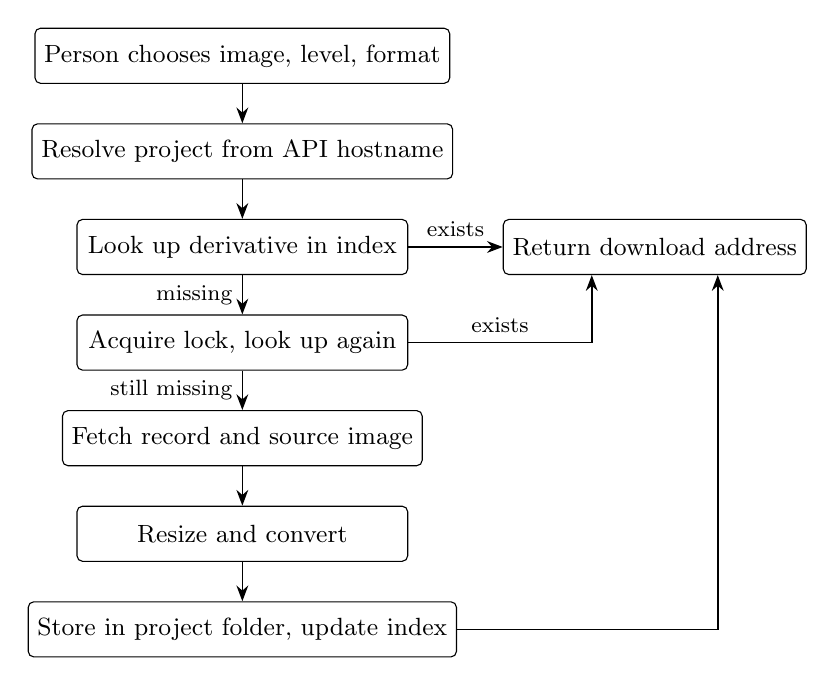
\begin{tikzpicture}[
      node distance=5mm and 12mm,
      box/.style={draw, rounded corners=2pt, align=center, font=\small,
                  minimum width=42mm, minimum height=7mm},
      side/.style={draw, rounded corners=2pt, align=center, font=\small,
                   minimum width=34mm, minimum height=7mm},
      arr/.style={-{Stealth[length=2mm]}, semithick}]
    \node[box] (req) {Person chooses image, level, format};
    \node[box, below=of req] (proj) {Resolve project from API hostname};
    \node[box, below=of proj] (idx) {Look up derivative in index};
    \node[box, below=of idx] (lock) {Acquire lock, look up again};
    \node[box, below=of lock] (fetch) {Fetch record and source image};
    \node[box, below=of fetch] (conv) {Resize and convert};
    \node[box, below=of conv] (store) {Store in project folder, update index};
    \node[side, right=of idx] (ret) {Return download address};
    \draw[arr] (req) -- (proj);
    \draw[arr] (proj) -- (idx);
    \draw[arr] (idx) -- node[left, font=\footnotesize] {missing} (lock);
    \draw[arr] (lock) -- node[left, font=\footnotesize] {still missing} (fetch);
    \draw[arr] (fetch) -- (conv);
    \draw[arr] (conv) -- (store);
    \draw[arr] (idx) -- node[above, font=\footnotesize] {exists} (ret);
    \draw[arr] (lock.east) -| node[pos=0.25, above, font=\footnotesize] {exists} ([xshift=-8mm]ret.south);
    \draw[arr] (store.east) -| ([xshift=8mm]ret.south);
  \end{tikzpicture}
  \caption{Path of a download request. A derivative that already exists
    is returned without contacting the project API or touching the
    source image.}
  \label{fig:workflow}
\end{figure}

\subsection{Project-Scoped Storage and Stable Addresses}

GRIDH projects follow a naming convention in which each project lives
at its own subdomain of the infrastructure's domain. The service
derives the project name from the hostname of the API address and
accepts it only if it matches that convention. The project name then
determines where files are written: every project has its own folder in
public storage, and within it a predictable path built from the image
identifier, the level and the format. The file keeps the base name of
the source file, so that what a person downloads is recognisably the
same object they were looking at.

Two consequences matter for users. First, the address of a derivative
is stable and can be shared. Second, each project's downloads form a
browsable public directory that is independent of the service: if the
service is switched off, the files it has produced remain available.

\subsection{Looking Up Without Searching}

Checking whether a file exists sounds trivial, but repeatedly
traversing directories becomes slow as the number of images grows. The
service therefore keeps a lightweight index in an SQLite database, with
one row per derivative keyed on project, image, level and format,
together with a checksum of the file. The index is treated as a hint,
not as the truth. When it reports a file, the service confirms that the
file is really on disk. If it is not, the stale row is removed and the
derivative is regenerated. An infrastructure maintained by a small team
will sooner or later have someone tidy a directory by hand, and the
system should recover from that without intervention.

\subsection{Simultaneous Requests}

When a project publishes a new image, several people may ask for the
same derivative within seconds of each other. Without care, each
request would see that the file is missing and start its own download
and conversion. The service takes a lock specific to the image and
level, and checks the index a second time once it holds the lock. The
first request does the work; the others wait briefly and then receive
the file the first one produced.

\section{Discussion: Whose Loop?}

\subsection{The Researcher's Loop: Resolution as Interpretation}

How much resolution is needed is not a technical question. It depends
on what one wants to see. A lecture slide, a reading of brushwork, a
comparison of compositions and a print for an exhibition call for
different images of the same object. Deciding among them requires
knowing the material and the argument one intends to make with it. This
is exactly the kind of situated, interpretive judgement that the
humanities are practised in, and it is the judgement that the service
leaves with the person.

The alternative designs each remove that judgement. Always serving the
original presumes that more data is better. Always serving a reduced
image presumes that the infrastructure knows what the researcher
needs. An adaptive system that guessed the appropriate size would hide
the decision altogether. Three named levels make the decision explicit
and make it cheap to revise: a person who finds the medium image
insufficient can ask for the full one, and the cost of having tried the
smaller one first is negligible.

\subsection{The Maintainer's Loop: Care and Limits}

The second human in the loop is the research engineer. The design
choices described above (compute once, verify the index against the
disk, accept only known hosts, keep projects apart) are not
optimisations for their own sake. They are what allows a small team to
offer an open service without being afraid of it. Infrastructure that
its maintainers do not trust tends to be closed down or locked away,
and that is a worse outcome for users than a service with three sizes.

There is also an environmental argument. Each derivative that is
reused instead of recomputed, and each download of a quarter of the
pixels in place of all of them, is a small saving in energy and
storage. Individually these are negligible. As a default embedded in
every project's interface they add up, and they reflect the position
that fidelity should be justified by use \citep{pendergrass2019}.

\subsection{The Project's Loop: Governance}

The third loop is the project. The service is deliberately organised
around projects, in storage layout, in naming and in the public
directory each project receives. This mirrors how responsibility for
the material is actually distributed. Whether a given collection should
be downloadable at full resolution is a question for those who know
its rights situation and the interests of the people connected to it
\citep{carroll2020}. A per-project structure does not answer that
question, but it gives the answer somewhere to live.

\subsection{Limitations}

We want to be explicit about what the prototype does not yet do,
because the tensions are instructive.

First, the service lets an operator state the project name explicitly
when an API address does not follow the usual convention. This is
convenient, and in the current implementation it also bypasses the
hostname check. Convenience for the operator and safety for the
infrastructure are in direct conflict here, and the check needs to
apply regardless of how the project is named before the service is
exposed more widely.

Second, the service currently places no upper bound on the pixel count
of a source image, on the reasoning that sources come from the
infrastructure's own storage and that documentation images are
legitimately enormous. The source is also read into memory in full.
Both are acceptable for trusted material at modest load and neither
would be for arbitrary input.

Third, the lock that prevents duplicate work lives inside a single
running process. It would not coordinate several server processes or
machines.

Fourth, the service has no notion of who is asking. It does not
authenticate, limit request rates, or distinguish a researcher from an
automated harvester. The fixed set of levels bounds the work any
requester can cause, to a small number of derivatives per image, but it
does not address bulk collection of the results. Given current
pressures on cultural heritage servers \citep{weinberg2025}, this is
the question we consider most urgent.

Finally, we have not yet studied how researchers actually use the
levels. Whether three is the right number, whether the labels are
understood as intended, and how often the full-resolution level is
really needed are empirical questions.

\section{Conclusion}

We have described a small piece of infrastructure and argued that its
most important property is a division of labour between human and
machine. The machine remembers what it has already made, keeps
projects apart and refuses to do the same work twice. The human decides
how much image is enough. Designing for that division required stating
openly that the needs of users and the needs of maintainers are
different, and treating neither as a constraint to be minimised.

Read through the theme of this conference, the lesson is that keeping
the humanities in the loop is not only a matter for systems that
classify or generate. It is equally a matter for the unglamorous layers
that decide what people are handed when they ask for a file. Future
work will address the limitations listed above, connect the service to
the download controls of GRIDH's image-based projects, and gather
evidence on how the resolution levels are used in research and
teaching.

\begin{acknowledgments}
  The service described here was developed at the Gothenburg Research
  Infrastructure in Digital Humanities (GRIDH), University of
  Gothenburg.
\end{acknowledgments}

\printbibliography

\end{document}
